\chapter{Orthogonalité, algorithme de Gram-Schmidt}
\label{chapter:Fr_22-orthogproj}


Nous avons étudié de nombreuses généralisations de $\R^2$ et 
$\R^3$ à des espaces vectoriels plus généraux (comme l'espace $\R^n$ ou l'espace des fonctions), mais dans chaque cas nous n'avons pas utilisé la géométrie du produit scalaire. Dans ce
chapitre, nous voulons étudier ce que la géométrie qui apparaît dans $\R^n$ grâce au produit scalaire.  

En fait, on peut ajouter un produit scalaire à tout espace vectoriel.
Par exemple, sur l'espace des fonctions continues dont le domaine est $[a,b]$, l'analogue du produit scalaire des vecteurs est le \stress{produit scalaire des fonctions} défini comme suit :
$$
\langle f, g \rangle = \int_a^b f(x)g(x)\;dx\,.
$$
C'est un sujet que l'on peut explorer dans un cours avanc\'e d'analyse. 
On peut également d\'efinir un produit scalaire sur l'espace des matrices $\M_{m\, n}$ comme suit: 
$$
\langle A, B \rangle = \tr (AB^T)\,.
$$
Mais encore une fois, l'étude de ce produit scalaire se fera dans un cours plus avancé.
Les produits scalaires ci-dessus possèdent un certain nombre de 
propriétés extrêmement intéressantes, mais il existe d'autres formes bilinéaires
qui codent différentes géométries (comme l'espace-temps) de manière plus précise.
Vous pouvez explorer ce sujet plus en détail dans des cours avanc\'es d'algèbre linéaire appliquée.



\section{Orthogonalit\'e}

Rappelons que deux vecteurs $\uu, \vv \in \R^n$ sont dits \emph{orthogonaux}\index{vecteurs orthogonaux} si leur
produit scalaire $\uu \cdot \vv$ est nul.  Le produit scalaire satisfait les propri\'et\'es suivantes:
\begin{itemize}
\item $\uu \cdot \uu \geq 0$, et $\uu\cdot\uu$ est nul si et seulement si $\uu = \zero$ (défini positif),
\item $\uu \cdot \vv = \vv \cdot \uu$ (symétrique);
\item $(a\uu + b\vv)\cdot(c\ww) = ac \uu \cdot \ww + bc \vv \cdot \ww$;
pour tous $a,b,c\in\R$ et $\uu,\vv,\ww \in \R^n$ (linéaire à gauche);
\item $(a\uu) \cdot (b\vv + c\ww) = ab\uu \cdot \vv + ac \uu \cdot \ww$.
(linéaire à droite).
\end{itemize}
\begin{myexample} Les vecteurs $(1,-1,0,1)$ et $(1,1,1,0)$ de $\R^4$ sont orthogonaux car 

$$(1,-1,0,1)\cdot(1,1,1,0)=1\cdot 1 + (-1) \cdot 1 + 0\cdot 1 + 1 \cdot 0=1-1=0\,.$$

\end{myexample}


\section{Ensembles de vecteurs orthogonaux}

La base standard de $\R^3$, \`a savoir $\set{(1,0,0), (0,1,0), (0,0,1)}$ (aussi notée $\set{\ee_1, \ee_2, \ee_3}$) consiste en des vecteurs qui sont deux-à-deux orthogonaux; c'est-à-dire 
$
\ee_i \cdot \ee_j = 0
$ pour tous $ i\not=j$.

Nous voulons généraliser cette idée, car cette base a (entre autres) la propriété très utile suivante : pour tout vecteur $\vv \in \R^3$, il est facile de trouver les scalaires $a,b,c$ tels que $\vv= a \,\ee_1 +b\,\ee_2+ c\,\ee_3$ --- il suffit de calculer $a=\vv\cdot \ee_1$ et  $b=\vv\cdot \ee_2$ et $c=\vv\cdot \ee_3$.

\begin{definition}
Un ensemble de vecteurs $\{\vv_1, \cdots, \vv_m\}$ de $\R^n$ est dit \emph{orthogonal} \index{ensemble orthogonal} si
 $$
\vv_i \cdot \vv_j = 0
$$
pour tout $1 \leq i < j \leq m$ et si $\vv_i\not=\zero$ pour tout $1 \leq i  \leq m$. Donc les vecteurs sont deux-à-deux orthogonaux et aucun vecteur n'est le vecteur nul.
\end{definition}

Remarque : si un ensemble orthogonal est constitué de vecteurs qui sont tous de norme $1$, alors l'ensemble est dit {\it orthonorm\'e}. C'est assez facile d'obtenir une ensemble orthonormé à partir d'un ensemble orthogonal : si $\{\vv_1, \cdots, \vv_m\}$ est orthogonal, alors 
$\{\frac{\vv_1}{\|\vv_1\|}, \dots, \frac{\vv_m}{\|\vv_m\|}\}$ est orthonormé.


\begin{myexample} La base standard de $\R^n$ est un ensemble orthogonal. (Elle est même orthonormée.) \end{myexample}

\begin{myexample} $\{ (1,0,0), (0,1,0), (1,0,1)\}$ n'est pas orthogonale même si deux de ses produits scalaires sont nuls.
En fait, le premier et le troisième vecteurs ne sont pas orthogonaux. \end{myexample}

Les ensembles orthogonaux vérifient également la propriété générale de Pythagore : si $\{\vv_1, \cdots, \vv_m\}$ est orthogonal, alors 
\begin{equation*} \|\vv_1 + \vv_2 +\cdots + \vv_m\|^2 =\|\vv_1\|^2 + \|\vv_2\|^2 +\cdots + \|\vv_m\|^2 \tag{$\star$}\,. \label{eqn:Pythag}
\end{equation*}

Prouvez-le par vous-même  (ce n'est pas très dur, rappelez-vous que $\|\vv\|^2= \vv\cdot \vv$).

Encore mieux, (et tout comme la base standard de $\R^n$) chaque ensemble orthogonal est linéairement indépendant :

\begin{theorem}[Les ensembles orthogonaux sont LI]\index{indépendance linéaire des ensembles orthogonaux}\label{theorem:orthogLI}
Tout ensemble orthogonal est linéairement indépendant.
\end{theorem}


\begin{proof}
Soit $\{\vv_1, \cdots, \vv_m\}$ un ensemble orthogonal et 
supposons qu'il existe des scalaires $a_1, \cdots, a_m\in\R$ tels que
$$
a_1\vv_1 + \cdots + a_m\vv_m = \zero.
$$
Prenez le produit scalaire avec $\vv_1$ des deux côtés. Le résultat doit être nul car le côté droit est $\zero\cdot\vv_1 = 0$. 
Cependant, du côté gauche, nous obtenons
$$
(a_1\vv_1 + \cdots + a_m\vv_m)\cdot\vv_1 = a_1 \vv_1 \cdot \vv_1 + a_2 0 + \cdots +a_m 0
$$
car $\vv_1 \cdot \vv_j = 0$ pour tout $j>1$ par orthogonalité. Ainsi $a_1\, \vv_1\cdot\vv_1=0$, et comme$\vv_1 \cdot \vv_1 \neq 0$
(car $\vv_1 \neq \zero$), on a que $a_1 = 0$.
En continuant de cette manière avec chacun des vecteurs $\vv_i$ à la place de $\vv_1$, on obtient $a_i=0$ pour
tout $i$. En conclusion, la relation de dépendance est triviale et notre ensemble $\{\vv_1, \cdots, \vv_m\}$ est bien linéairement indépendant.
\end{proof}

Il s'agit là d'un r\'esultat important, car il nous dit que:
\begin{itemize}
\item tout sous-ensemble orthogonal de $\R^n$ possède AU PLUS $n$ éléments (sinon l'ensemble ne pourrait pas être LI);
\item tout sous-ensemble orthogonal de $n$ vecteurs de $\R^n$ est une base de $\R^n$, appelée \defn{base orthogonale}.
\end{itemize}
De plus, la preuve nous a donné un moyen {\it très simple} de calculer les
coordonnées d'un vecteur par rapport à une base orthogonale.

\begin{theorem}[Coordonnées par rapports à une base orthogonale]\label{expansion}\index{coordonnées relatives à une base orthogonale}
Supposons que $\{\ww_1, \cdots, \ww_m\}$ soit une base orthogonale d'un sous-espace $W$ de $\,\R^n$.
Alors tout vecteur $\ww \in W$ peut s'écrire comme suit
\begin{equation*}
\ww = \left( \frac{  \ww \cdot\ww_1}{\Vert \ww_1 \Vert^2} \right) \ww_1 +
  \left( \frac{\ww \cdot\ww_2}{\Vert \ww_2 \Vert^2} \right) \ww_2 + \cdots +
 \left( \frac{\ww \cdot\ww_m}{\Vert \ww_m \Vert^2} \right) \ww_m
 \tag{$\star\star$}\label{expand} \,.\end{equation*}
\end{theorem}

Les coefficients devant les vecteurs $\ww_1, \dots, \ww_m$ obtenus ci-dessus sont les coordonnées de $\ww$ dans la base ordonnée $\set{\ww_1, \dots, \ww_m}$. Ces coefficients sont souvent appelés les \defn{coefficients de Fourier} de $\ww$ par rapport à cette base orthogonale.

Le fait important ici est:  pour écrire $\ww$ comme combinaison linéaire des vecteurs d'une base orthogonale, il existe une formule simple qui vous donne la réponse, alors que normalement vous devez réduire par rapport aux lignes une matrice, ce qui est assez long... 

\begin{proof}
Puisque $\{\ww_1, \cdots, \ww_m\}$ est une base de $W$, nous savons qu'il existe
des scalaires $a_1, \cdots, a_n\in\R$ tels que 
$$
\ww = a_1\ww_1 + \cdots + a_n\ww_n\,.
$$
Prenons maintenant le produit scalaire avec $\ww_i$ des deux côtés. L'égalité se simplifie comme suit :
$$
\ww \cdot \ww_i = a_i \,\ww_i \cdot \ww_i\,,
$$
ce qui donne l'expression voulue pour les coefficients :
$$
a_i = \frac{\ww \cdot \ww_i }{\ww_i \cdot \ww_i} = \frac{\ww_i \cdot \ww }{\Vert \ww_i\Vert^2}
$$
(Notez qu'on peut diviser par $|| \ww_i||^2$ puisque $\ww_i\neq\zero$ par définition d'ensemble orthogonal.)
\end{proof}

\begin{myprob} Exprimez le vecteur $(1,6,7)$ comme combinaison lin\'eaire des vecteurs $(1,2,1)$, $(1,0,-1)$
et $(1,-1,1)$.

\begin{mysol} On remarque que ces trois derniers vecteurs sont orthogonaux, et donc forment
une base pour $\R^3$.  Par conséquent, le théorème s'applique et nous déduisons que
$$
\mat{1\\6\\7} = \frac{20}{6}\mat{1\\2\\1} + \frac{-6}{2}\mat{1\\0\\-1} + \frac{2}{3}\mat{1\\-1\\1}\,.
$$
(Vérifiez que c'est bien vrai !)
\end{mysol}\end{myprob}


\begin{myexample}
Soit $W=\set{(x,y,z,w) \in \R^4 \st x-y-z+w=0}$. Nous savons que $W$ est un sous-espace de $\R^4$. Montrons que $\dim W=3$. On remarque que $W=\ker(\bmatrix1&-1&-1&1 \endbmatrix)$ et que le rang de $\bmatrix1&-1&-1&1 \endbmatrix$ est 1. Donc, par le Théorème du rang \ref{corollary:ranknull} : $$\dim W= \dim \ker(\bmatrix1&-1&-1&1 \endbmatrix)=4-\rank(\bmatrix1&-1&-1&1 \endbmatrix)=3\,.$$

Considérons maintenant les trois vecteurs  $\ww_1=(1,1,1,1), \ww_2=(1,-1,1,-1),\ww_3=(1,1,-1,-1)$.\footnote{Ne vous inquiétez pas à propos de la façon dont nous avons trouvé les vecteurs $\ww_1, \ww_2, \ww_3$, nous verrons une méthode plus tard pour y arriver : l'\emph{algorithme de Gram-Schmidt}} Il est facile de vérifier qu'ils sont dans $W$ et que $\set{\ww_1,\ww_2,\ww_3}$ est un ensemble orthogonal, donc linéairement indépendant. Puisque nous avons trois vecteurs linéairement indépendants dans le sous-espace $W$ de dimension 3, il suit que $\set{\ww_1,\ww_2,\ww_3}$ est une base orthogonale de $W$.

Ensuite, considérons $\ww = (1,2,3,4)$ qui est bien un vecteur de $W$ (vous pouvez le vérifier). Utilisons notre théorème pour écrire $\ww$ comme une combinaison linéaire de
 $ \ww_1,\ww_2$ et $\ww_3$.



Un calcul simple donne
$$
\frac{\ww\cdot \ww_1}{\|\ww_1\|^2} = \frac{10}{4} = \frac52
$$
$$
\frac{\ww\cdot \ww_2}{\|\ww_2\|^2} = \frac{-2}{4} = -\frac12
$$
$$
\frac{\ww\cdot \ww_3}{\|\ww_3\|^2} = \frac{-4}{4} = -1
$$

Donc on peut conclure que
$$
\ww = \frac52\ww_1 - \frac12\ww_2 - \ww_3\,.
$$
(Vous pouvez vérifier directement que c'est bien vrai si vous le souhaitez).

Comparez cela avec la méthode de réduction par rapport aux lignes :
$$ \mat{\ww_1 &\ww_2 &\ww_3&|&\ww}=
\mat{
1 & 1  & 1 &   |& 1\\
1 & -1 & 1 &   |& 2\\
1 & 1  & -1 &   |& 3\\
1 & -1 & -1 &   |& 4}
\sim
\mat{
1 & 1  & 1 &   |& 1\\
0 & -2 & 0 &   |& 1\\
0 & 0  & -2 &   |& 2\\
0 & -2 & -2 &  |& 3}
\sim
\mat{
1 & 0  &  1 &   |& \frac32\\
0 & 1 &   0 &  |& -\frac12\\
0 & 0  & -2 &   |& 2\\
0 & 0 & -2 &   |& 2}
$$
$$
\sim
\mat{
1 & 0  &  0 &   |& \frac52\\
0 & 1 &   0 &   |& -\frac12\\
0 & 0  & 1 &   |& -1\\
0 & 0 & 0 &   |& 0}
\sim
\mat{
1 & 0  &  0 & 0 & |& \frac52\\
0 & 1 &   0 & 0 & |& -\frac12\\
0 & 0  & 1 & 0 & |& -1\\
0 & 0 & 0 & 1 & |& 0}\,.
$$
On obtient bien la même réponse, mais cette technique a demandé bien plus d'efforts !
\end{myexample}

\standout{N.B.: \stress{si} vous avez une base orthogonale, alors certains calculs seront beaucoup plus faciles.  \stress{Mais si vous n'avez pas de base orthogonale}, alors vous devez utiliser les\ \og anciennes\ \fg\  techniques, c'est-à-dire la réduction par rapport aux lignes par exemple, laquelle est beaucoup plus lente... mais au moins elle marche !}

\section{Projection orthogonale : plusieurs usages d'une même formule... }

Dans cette section, regardons à nouveau le côté droit de l'équation ($\star\star$) dans le Théorème \ref{expansion}. En fait, le côté droit aurait aussi tout à fait du sens {\it même si $\ww$ n'était pas dans $W$ !}  C'est là l'idée derrière la projection orthogonale sur un sous-espace.

En effet, par exemple regardez le tout premier terme de cette somme : 
$$\left( \frac{ \ww \cdot\ww_1}{\Vert \ww_1 \Vert^2} \right) \ww_1\,.$$ 
Nous reconnaissons qu'il s'agit bien de la projection du vecteur $\ww$ sur le vecteur $\ww_1$ (rappel : nous avions étudié la projection orthogonal dans le contexte de $\R^3$, cf. la Section \ref{projR3} à la page \pageref{projR3}). Les autres termes sont également des projections du même vecteur $\ww$ sur les autres vecteurs $\ww_2, \dots, \ww_m$. Ainsi, l'expression du côté droit de l'équation ($\star\star$) \`a la page \pageref{expand} est une somme des projections de $\ww$ sur les vecteurs (orthogonaux) $\ww_1, \dots, \ww_m$, lesquels forment une base du sous-espace $W$.  Il n'est donc pas {\it complètement} \'etrange de considérer cette expression comme la projection orthogonale de $\ww$ sur le \underbar{\emph{sous-espace}} $W$. (Attention : on ne projette pas un vecteur sur n'importe quel type de sous-ensemble, on projette seulement sur un sous-espace.)




\begin{definition}[Projection orthogonale sur un sous-espace]\label{projdef}\index{projection orthogonale}
Soit $W$ un sous-espace de $\R^n$ et soit $\{ \ww_1,\ww_2, \ldots, \ww_m\}$ une base \underbar{\stress{orthogonale}} de $W$.    
Alors pour tout vecteur $\vv \in \R^n$, la \stress{projection orthogonale de $\vv$ sur $W$} est le vecteur défini comme suit :
$$
\proj_W(\vv) = \left(\frac{\vv\cdot \ww_1}{\Vert \ww_1\Vert^2}\right) \ww_1 + \cdots 
+ 
\left(\frac{\vv\cdot \ww_m}{\Vert \ww_m\Vert^2}\right)\ww_m\,.
$$
\end{definition}

Regardez la Figure \ref{fig:19.1} pour visualiser ce qui se passe, du moins en dimension $3$ puisque la plupart d'entre nous ne sommes que des êtres de dimension inf\'erieure...
\begin{figure}
\begin{center}
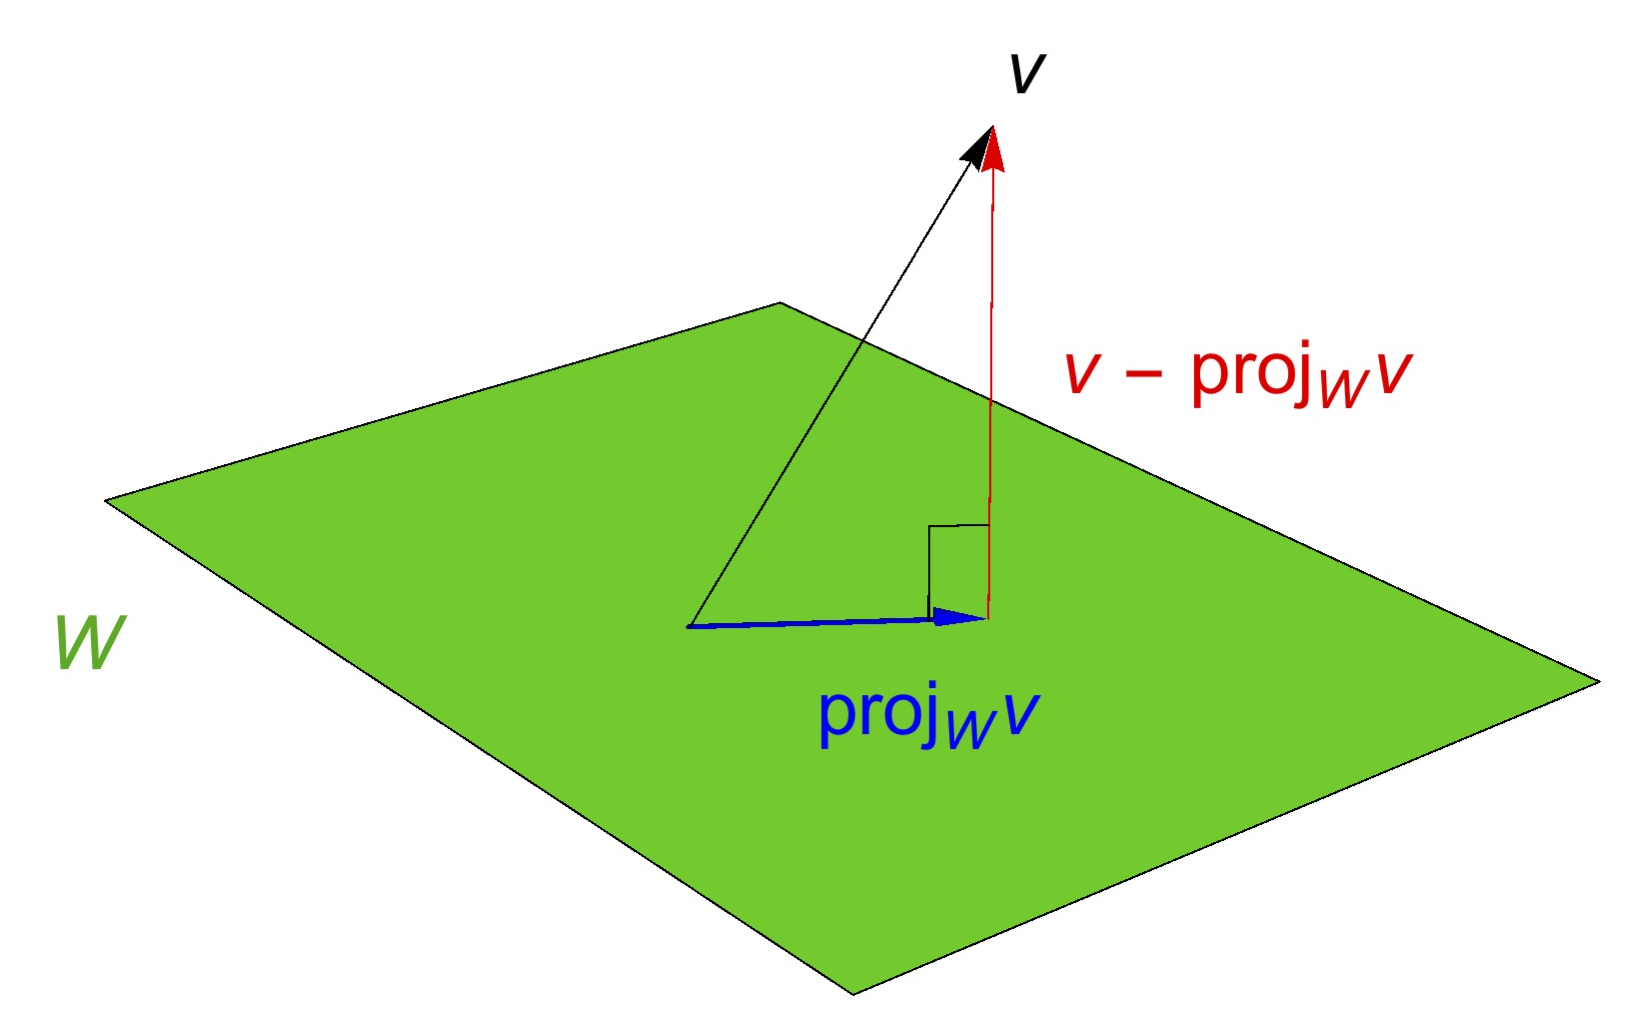
\includegraphics[scale=.2] {projW.jpg}~\\[1cm]
\end{center} 
\vglue-1cm
\caption{La projection orthogonale de $\vv$ sur le sous-espace $W$.}\label{figure:othogproj}\label{fig:19.1}
\end{figure}

Maintenant que la curiosité de votre esprit a été attisée, vous vous posez sans doute les deux questions suivantes :
\begin{enumerate}

\item {\it N'importe quel sous-espace admet-t-il une base orthogonale ?} Car la formule en a besoin...\label{goodquestion1}

\item {\it Si je calcule cette projection avec 2 bases orthogonales différentes, que se passe-t-il ? Je vais sûrement obtenir des réponses différentes, non ?\!? Du moins, les coordonnées seront différentes...}
\end{enumerate}
 
\medskip

Après avoir étudié un exemple, nous répondrons à la deuxième question; puis plus tard nous nous attaquerons à la première question, lorsque nous aurons introduit l'algorithme de Gram-Schmidt.


\begin{myexample}
Regardons à nouveau le sous-espace $W=\set{(x,y,z,w) \in \R^4 \st x-y-z+w=0}$. Par ce qui précède, nous savons que les 3 vecteurs $\ww_1=(1,1,1,1), \ww_2=(1,-1,1,-1)$ et $ \ww_3=(1,1,-1,-1)$ forment une base orthogonale pour $W$, et que le vecteur $\vv = (1,2,3,5) \notin W$ est projeté sur le vecteur :
$$
\proj_W(\vv) = \frac{11}4\ww_1 - \frac34\ww_2 - \frac{5}{4}\ww_3=\frac14\mat{3\\ 9\\ 13\\ 19}\in W\,.
$$
(Si vous le souhaitez, vous pouvez vérifier que $\frac14(3, 9, 13, 19)\in W$; il suffit de montrer que ce vecteur satisfait l'équation $x-y-z+w=0$.)

{\bf N.B.:} \underbar{Vous ne devez pas changer la longueur du vecteur de cette réponse!} C'est-à-dire : il ne faut pas changer le coefficient $\frac14$ devant le vecteur. Il s'agit d'une erreur très, très courante à ce stade. Vous pouvez changer la longueur des vecteurs d'une base orthogonale, mais vous ne pouvez pas changer la longueur du vecteur projection, c'est une réponse fixe !

De plus, comme le suggère la Figure \ref{figure:othogproj},
le vecteur $\vv-\proj_W(\vv)=\frac14(1, -1, -1, 1)$ est en fait orthogonal à tout vecteur de $W$ (cette idée était déjà le cas dans $\R^3$, voir pages \pageref{propOrthogProj} et \pageref{orthoprojonvector}). Pour montrer cela, regardez à nouveau l'équation définissant $W$ : elle nous dit que $(x,y,z,w) \in W$ si et seulement si 
$$ 0=x-y-z+w=(x,y,z,w)\cdot(1, -1, -1, 1)\,.$$ Donc tout vecteur de $W$ {\it est} bien orthogonal à $\vv-\proj_W(\vv)$.
\end{myexample}

\standout{\it Ceci arrive toujours : le vecteur $\vv-\proj_W(\vv)$ est bien orthogonal à n'importe quel vecteur de $W$. De plus, comme les Figures \ref{orthoprojonvector} et \ref{figure:othogproj} le suggèrent, le vecteur $\proj_W(\vv)$ est en fait {\it le  vecteur le plus proche de $\vv$ parmi tous les vecteurs de $W$}. 

Une autre façon de le dire: le vecteur $\proj_W(\vv)$ est la {\it meilleure approximation de $\vv$ par un vecteur de $W$}.}

Montrons que ceci est vrai.
\begin{theorem}[La meilleure approximation]\index{projection orthogonale} \label{orthogproj}
Soit $W$ un sous-espace de $\R^n$ et soit $\vv \in \R^n$. Alors on a :

\begin{enumerate}[(1)]
\item $\proj_W(\vv) \in W$;
\item $\vv - \proj_W(\vv)$ est orthogonal \`a tout vecteur de $W$;
\item $\proj_W(\vv)$ est la meilleur approximation de $\vv$ par un vecteur de $W$;
\item le vecteur $\proj_W(\vv)$ est l'\underbar{unique} vecteur de $\R^n$ qui satisfait (1) et (2).
\end{enumerate} 

\end{theorem}



Remarque : la propriété (4) nous dit que la projection orthogonale
est uniquement caractérisée par les deux propriétés (1) et (2).


\begin{proof} 
\begin{enumerate}[(1)]
	\item Cette partie est facile à montrer : utilisez la formule dans la Définition \ref{projdef}. Le vecteur $\proj_W(\vv)$ est une combinaison linéaire de vecteurs du sous-espace $W$ et doit donc appartenir à $W$.

	\item Comment pourrions-nous montrer qu'un vecteur est orthogonal à chaque vecteur de $W$ ? Il y a une infinité de vecteurs dans un sous-espace (du moins dans la plupart d'entre eux)...  C'est là que les bases vont être très utiles : pour «~rendre fini l'infini~» ! 

Supposons donc que $\{\ww_1, \cdots, \ww_m\}$ soit la base orthogonale pour $W$ que nous avons utilisée pour définir la projection. Chaque vecteur $\uu\in W$ est alors combinaison linéaire des $\ww_1, \cdots, \ww_m $; c'est-à-dire que $u$ s'écrit
 $$\uu =a_1 \ww_1 +\cdots + a_m \ww_m$$ pour certains scalaires $a_1, \cdots, a_m\in\R$. 
 Donc si l'on arrive à montrer que $(\vv-\proj_W(\vv))\cdot \ww_i=0$ pour tout $1\le i \le m$, alors le tour est joué (en notant $\ww=\proj_W(\vv)$ dans ce qui suit) :
\vglue-.4cm
\begin{align*} 
(\vv-\ww) \cdot \uu &=(\vv-\ww)\cdot (a_1 \ww_1 +\cdots + a_m \ww_m) \\
&=a_1((\vv-\ww)\cdot \ww_1) +\cdots +a_1((\vv-\ww)\cdot \ww_m)\\
&=a_1(0) +\cdots +a_1(0)\\&=0\,.
\end{align*}
(Notez que nous n'avons utilisé qu'une seule propriété de $\{\ww_1, \cdots, \ww_m\}$ : le fait qu'il engendre $W$. Donc en fait, on a même montré quelque chose de plus général : si un vecteur $\vv$ est orthogonal à un {\it ensemble g\'en\'erateur} de $W$, alors $\vv$ est orthogonal à tout vecteur du un sous-espace $W$ !)
Il reste donc à montrer que $(\vv-\ww)\cdot \ww_i=0$ pour tout $1\le i \le m$. On calcule : 
\begin{align*}
 (\vv-\ww)\cdot\ww_i  &=
(\vv - (\frac{\vv\cdot \ww_1}{\Vert \ww_1\Vert^2}\ww_1 + \cdots 
+ 
\frac{\vv\cdot \ww_m}{\Vert \ww_m\Vert^2}\ww_m))\cdot \ww_i \\
 &= \vv \cdot \ww_i - \frac{\vv\cdot \ww_1}{\Vert \ww_1\Vert^2}\ww_1 \cdot \ww_i - \cdots - \frac{\vv\cdot \ww_m}{\Vert \ww_m\Vert^2}\ww_m \cdot \ww_i\\
&= \vv \cdot \ww_i - \frac{\vv\cdot \ww_i}{\Vert \ww_i\Vert^2}\ww_i \cdot \ww_i
\end{align*}

puisque tous les autres produits scalaires entre $\ww_i$ et $\ww_j$ sont nuls ;
et ce dernier terme donne :
$$
 = \vv \cdot \ww_i - \frac{\vv\cdot \ww_i}{\Vert \ww_i\Vert^2}\Vert \ww_i \Vert^2 = 0\,.
$$
Ceci est vrai pour chaque $i = 1,2,\cdots, m$, et nous pouvons donc conclure que $\vv-\ww$ est orthogonal à tout vecteur de $W$, ce qui montre que (2) est vrai.


	\item On pose comme précédemment $\ww = \proj_W(\vv)$.  Pour prouver que c'est le vecteur le plus proche
dans $W$ de $\vv$, soit $\ww' \in W$ un autre vecteur quelconque dans $W$.
Alors on a
$$
\Vert \vv- \ww' \Vert^2 = \Vert (\vv - \ww) + (\ww - \ww') \Vert^2
$$
Or, d'une part $\vv-\ww$ est orthogonal à tout vecteur de $W$, et d'autre part $\ww - \ww'$ est dans $W$ (puisque $W$ est un sous-espace et que $\ww$ et $\ww'$ appartiennent tous deux à $W$). Donc les deux vecteurs $\vv - \ww$ et $\ww - \ww'$
sont orthogonaux, et par le Théorème de Pythagore (\ref{eqn:Pythag}) page \pageref{eqn:Pythag}, nous avons l'égalité:
$$
\Vert \vv- \ww' \Vert^2 = \Vert (\vv - \ww)\Vert^2 + \Vert(\ww - \ww') \Vert^2\,.
$$
Mais ceci est $\geq \Vert (\vv - \ww)\Vert^2$
car on a toujours $ \Vert(\ww - \ww') \Vert^2\geq 0$, et donc nous avons montré que (3) est vrai.

	\item Cette partie est également simple. Supposons maintenant que deux vecteurs $\ww,\ww'$ satisfont les propriétés (1) et (2) ci-dessus, à savoir :

\begin{itemize}
\item $\ww, \ww' \in W$
\item $\vv - \ww$ et $\vv-\ww'$ sont chacun orthogonal \`a tout vecteurs de $W$.
\end{itemize}

Alors, $\ww- \ww'\in W$ puisque $W$  est un sous-espace. Mais regardez : $$\ww- \ww'= (\vv-\ww')-(\vv - \ww).$$ Or, la somme -- ou la différence -- de deux vecteurs qui sont tous deux orthogonaux à chaque vecteur de $W$ sera à nouveau orthogonale à chaque vecteur de $W$. \footnote{Je ne sais pas pour vous, mais je commence à en avoir assez d'écrire \ \og est orthogonal à chaque vecteur de $W$\ \fg. Nous allons donc bientôt donner un nom à l'ensemble de tous les vecteurs orthogonaux à chaque vecteur de $W$. Nous l'appellerons $W^\perp$ --- voir Chapitre \ref{chapter:Fr_23-orthogcomp}.} Donc le vecteur $\ww- \ww'$ est orthogonal à chaque vecteur de $W$, y compris $\ww- \ww'$ lui-même ! Cependant, le seul vecteur orthogonal à lui-même est le vecteur nul, donc $\ww- \ww'=\zero$, ce qui donne bien l'unicité voulue $\ww= \ww'$.

Ceci montre bien qu'il n'existe qu'un seul vecteur ayant les propriétés (1) et (2) ci-dessus, à savoir $\proj_W(\vv)$.
\end{enumerate}
\end{proof}

Notez que la propriété (3) ci-dessus de la projection orthogonale est extrêmement utile dans de nombreux domaines. Elle constitue une partie importante de la base mathématique du traitement moderne du signal. Elle est utilisée dans presque toutes les méthodes quantitatives pour l'ajustement optimal de la courbe des données. Nous en présentons un exemple dans la Section \ref{leastsquares}, avec ce qu'on appelle l'\emph{approximation des moindres carrés}. 


L'idée de base est que nous disposons souvent d'un sous-espace $W$ (dans un espace vectoriel de signaux, par exemple) et d'un vecteur $\vv$ dont nous ne sommes pas certain qu'il appartienne à notre sous-espace $W$. Nous souhaitons ne traiter que les vecteurs de $W$\kern-2pt, donc nous projetons notre vecteur $\vv$ sur $W$ et nous traitons sa projection à la place de lui-même. 

Par exemple, pour faire simple, disons sur votre téléphone portable, lorsque vous prenez une photo et que vous souhaitez l'envoyer à un ami, la photo est capturée, stockée et traitée comme un vecteur dans un espace de grande dimension ($\R^n$ pour un certain nombre $n$ très grand). Cependant, au lieu d'envoyer toutes les entrées du vecteur, on projette le vecteur (orthogonalement) sur un sous-espace beaucoup plus petit -- avec une base orthogonale propre au protocole utilisé -- et ensuite on transmet d'un téléphone à l'autre uniquement les coefficients de Fourier, lesquels sont beaucoup moins nombreux que les $n$ coefficients de l'espace de départ. Sur le téléphone de votre ami qui reçoit les coefficients de Fourier, on peut ensuite utiliser la même base orthogonale pour restituer la projection à l'aide des coefficients de Fourier, obtenant ainsi une approximation (plus ou moins précise, en fonction de $\dim W$ et de $n$) de l'image que vous aviez envoyée.

La partie (4) ci-dessus semble inoffensive jusqu'à ce qu'on se rappelle que la Définition \ref{projdef} (page \pageref{projdef}) {\it semblait} dépendre d'un choix de base orthogonale. Donc en fait, ce que la partie (4) dit, c'est que les différentes formules que l'on obtient en utilisant différentes bases orthogonales pour calculer la projection donnent toutes exactement la même réponse finale! Wow ! Ceci répond à notre deuxième question !

\section{Bases orthogonales : l'algorithme de Gram-Schmidt}\label{section:Gram-Schmidt}

Jusqu'à présent, nous avons supposé implicitement que chaque sous-espace $W$ de $\R^n$ {\it admet} une base orthogonale. Est-ce vrai ? En fait oui, et encore même mieux, il existe un algorithme simple qui transforme n'importe quelle base de $W$ en une base orthogonale de $W$ !\!!


 

Supposons que $\set{\uu_1, \cdots, \uu_m }$ soit une base quelconque de $W$.  Nous voulons trouver une base orthogonale pour $W$.

L'idée géométrique est assez simple : commencez avec votre premier vecteur $\ww_1 = \uu_1$.
Prenez ensuite $\ww_2 = \uu_2 - \proj_{\uu_1}(\uu_2)$. Par ce qui précède, vous avez que $\ww_2$ est orthogonal à $\ww_1$, et on voit que $\ww_1$ appartient bien à $W$ (il est même combinaison linéaire de $\uu_1$
et $\uu_2$).  Continuez ainsi de suite à construire $\ww_i$ en soustrayant $\uu_i$ à sa projection sur le sous-espace $\spn\{\ww_1, \dots, \ww_{i-1}\}$. Lorsque vous aurez atteint $i=m=\dim(W)$, vous aurez construit une base orthogonale $\{\ww_1, \dots, \ww_{m}\}$ de $W$.

\begin{theorem}[L'algorithme de Gram-Schmidt]\index{algorithme de Gram-Schmidt}\label{theorem:GS}
Soit $\set{\uu_1, \cdots, \uu_m }$ une base {\it quelconque} de $W$.  On d\'efinit les vecteurs et sous-espaces suivants:
\begin{itemize}
\item $\ww_1 = \uu_1$  and $V_1 = \spn\{\ww_1\}$;
\item $\ww_2 = \uu_2 - \proj_{V_1}(\uu_2)$ and $V_2 = \spn\{\ww_1,\ww_2\}$;
\item $\ww_3 = \uu_3 - \proj_{V_2}(\uu_3)$ and $V_3 = \spn\{\ww_1,\ww_2,\ww_3\}$;
\item $\cdots$
\item $\ww_m = \uu_m - \proj_{V_{m-1}}(\uu_m)$ et $V_m = \spn\{\ww_1,\cdots,\ww_m\}$.
\end{itemize}
Alors $W = V_m$ et   
$\{\ww_1,\cdots,\ww_m\}$ est une base orthogonale pour $W$.

\medskip
Exprimés plus en détail, les vecteurs sont :

\begin{itemize}
\item $\ww_1 = \uu_1$;
\item $\ww_2 = \uu_2 - \proj_{\ww_1}(\uu_2)$;
\item $\ww_3 = \uu_3 - \proj_{\ww_1}(\uu_3)-\proj_{\ww_2}(\uu_3)$;
\item $\cdots$
\item $\ww_m = \uu_m - \sum_{i=1}^{m-1}\proj_{\ww_{i}}(\uu_m)$.
\end{itemize}
Alors $\{\ww_1,\cdots,\ww_m\}$ est une base orthogonale pour $W$.

Enfin, on peut normaliser cette base (\textit{i.e.} rendre la norme de chaque vecteur de la base \'egale \`a 1) en divisant les vecteurs par leur norme. On a alors
une base orthonormée de $W$.
\end{theorem}

Remarquez qu'à chaque étape, les vecteurs de l'ensemble g\'en\'erateur de $V_i$ sont orthogonaux, ce qui signifie qu'il est facile de calculer la projection sur
$V_k$.  En fait, on a $V_k = \spn\{\uu_1 , \cdots, \uu_k\}$ ; c'est à dire l'enveloppe lin\'eaire engendr\'ee par $\{\ww_1, \dots, \ww_k\}$ est la même que celle engendr\'ee par les vecteurs de l'ensemble original $\{\uu_1, \dots, \uu_k\}$, pour n'importe quel $1\leq k \leq m$.

\medskip
Par ailleurs, notez qu'on pourrait commencer par un  ensemble \emph{g\'en\'erateur} $\set{\uu_1,\cdots, \uu_p}$ de $W$ (plutôt qu'une base) et appliquer le même algorithme de Gram-Schmidt. Alors on obtiendrait un ensemble $\{\ww_1,\cdots,\ww_p\}$, et les  vecteurs {\it non nuls} de cet ensemble formeraient une base orthogonale de $W$ ! Voir Exercice~\ref{prob19.6}.

\begin{myexample}\label{example:GS} Exécutons l'algorithme de Gram-Schmidt sur l'ensemble 
$$\{ (1,0,0,1), (1,1,1,0), (2,1,-1,1)\}\,.
$$

(Vous pouvez vérifier que c'est bien une base du sous-espace $W=\sp{ (1,0,0,1), (1,1,1,0), (2,1,-1,1)}=\set{(x,y,z,w)\in \R^4\st x - y - w = 0}$.\footnote{Nous avons vu comment faire cela à la fin du Chapitre \ref{chapter:Fr_17-homogsystems}.})


On commence par poser
$$
\ww_1 = (1,0,0,1)\,,
$$
puis on calcule
\begin{align*}
\ww_2 &= \uu_2 - \proj_{\ww_1}(\uu_2)\\
&= \uu_2 - \frac{\uu_2\cdot \ww_1}{\|\ww_1\|^2}\ww_1 \\
&= (1,1,1,0) - \frac{1}{2}(1,0,0,1) = \left(\frac12,1,1,-\frac12\right). 
\end{align*}

(Avant de continuer, c'est toujours une bonne idée de vérifier qu'on a bien $\ww_1\cdot \ww_2 =0$ ! C'est pour se rassurer un peu qu'on n'a pas fait d'erreur de calcul... Vérifiez-le !).
Et, dans cet exemple, il ne reste qu'une autre étape \`a faire:

\begin{align*}
\ww_3 &= \uu_3 - \frac{\uu_3\cdot \ww_1}{\|\ww_1\|^2}\ww_1 - \frac{\uu_3\cdot \ww_2}{\|\ww_2\|^2}\ww_2\\
&= (2,1,-1,1) - \frac{3}{2} (1,0,0,1) - \frac{1/2}{5/2}
\left(\frac12,1,1,-\frac12\right) \\
&= (2,1,-1,1) -\left(\frac32,0,0,\frac32\right) - \left(\frac1{10}, \frac15
 , \frac15, -\frac1{10}\right)\\
&= \frac25(1, 2 , -3 , -1)\,.
\end{align*}
Nous pouvons alors voir que $\{\ww_1,\ww_2,\ww_3\}$ est effectivement orthogonal (c'est toujours une bonne idée de le vérifier). \footnote{Aussi, si vous avez le temps, c'est aussi une très bonne idée de vérifier que vos vecteurs $\ww_1,\ww_2,\ww_3$ appartiennent bien à $W$ -- ce qui est bien le cas ici ! Ici, c'est facile, car nous avons une description simple de $W$, à savoir  $W=\set{(x,y,z,w)\in \R^4\st x - y - w = 0}$, mais dans d'autres cas cette vérification peut être un peu plus longue...}  De plus,
en regardant nos calculs plus attentivement, nous pouvons voir qu'en effet,
chaque vecteur $\ww_i$ est bien dans l'enveloppe lin\'eaire engendr\'ee par les vecteurs originaux $\uu_1, \dots, \uu_i$. 
La base orthogonale résultante est alors la suivante :
$$
\left\{ (1,0,0,1), \frac12(1,2,2,-1), \frac25(1,2,-3,-1)\right\}\,.
$$  

\begin{remark} Nous simplifierons souvent nos résultats à la fin en multipliant les vecteurs 
$\ww_i$ par un scalaire convenable, de fa\c{c}on \`a éviter les fractions. Dans l'exemple pr\'ec\'edent, on peut donner le résultat suivant :
$$
\{ (1,0,0,1), (1,2,2,-1), (1,2,-3,-1)\}\,,
$$
lequel est bien un ensemble orthogonal, et il a le bon goût de ne pas avoir de fractions. Donc il
pourrait être
plus facile à utiliser si vous deviez calculer une autre projection par exemple.
\end{remark}

\medskip
Enfin, si l'on veut vraiment une base \emph{orthonormée}, il faut diviser chacun de ces vecteurs par leur norme.  Pour l'exemple pr\'ec\'edent, comme 
$
\Vert (1,0,0,1) \Vert = \sqrt{2}$,  que $\Vert  (1,2,2,-1) \Vert =   \sqrt{10}$, et que $ \Vert  (1,2,-3,-1) \Vert =   \sqrt{15} $, on obtient la base orthonormée suivante :
$$
\left\{ \frac{\sqrt{2}}{2}(1,0,0,1), \frac{\sqrt{10}}{ 10 }(1,2,2,-1), \frac{\sqrt{15}}{15}(1,2,-3,-1)\right\}\,.
$$
(V\'erifiez-le!) Par contre, pour les bases orthonormées, on ne peut pas changer la norme à notre guise pour enlever les fractions puisqu'on veut que la norme de chaque vecteur soit égale à $1$ (c'est une contrainte assez forte !).
\end{myexample}



\begin{myexample}\label{Wagain} Calculez la meilleure approximation de $\vv = (1,2,3,4)$ dans $W$, où
$$
W = \spn\{(1,0,0,1), (1,1,1,0), (2,1,-1,1)\}=\set{(x,y,z,w)\in \R^4\st x - y - w = 0}\,.
$$

Utilisons l'exemple précédent.  Nous savons déjà qu'une
base orthogonale pour $W$ est 
$$
\{  (1,0,0,1),  (1,2,2,-1),  (1,2,-3,-1)\}\,.
$$
Notons ces vecteurs respectivement $\nn_1$, $\nn_2$, $\nn_3$.
On a alors :
\begin{align*}
\proj_W(\vv) &= \frac{\vv\cdot\nn_1}{\|\nn_1\|^2} \nn_1 +  \frac{\vv\cdot\nn_2}{\|\nn_2\|^2} \nn_2 + \frac{\vv\cdot\nn_3}{\|\nn_3\|^2} \nn_3 \\  
&= \frac{5}{2}  (1,0,0,1) + \frac{7}{10} (1,2,2,-1)  -\frac{8}{15}(1,2,-3,-1)\\
&=  \frac{1}{3}(8,1,3,7).
\end{align*}

Si vous avez le temps, vérifiez que la réponse appartient bien à $W$. Ici c'est facile puisque nous avons une description simple de $W$. \footnote{ Si vous avez le temps, vous devriez également vérifier que le vecteur $(1,2,3,4)-\frac{1}{3}(8,1,3,7)=\frac13(-5,5,0,5)$ est orthogonal à tout vecteur de $W$. C'est bien le cas, puisque $\frac13(-5,5,0,5)\cdot (x,y,z,w)=-\frac53 (x-y-w)=0 $ \`a chaque fois que $(x,y,z,w)\in W$ ! }
\end{myexample}


